\title{Laboratory 1 - Fluids Labs}
\author{
        Sergio M. Vanegas A.\\
        Francesco de Pas\\
                Department of Mathematics\\
        Polimi---Politecnico di Milano\\
        Milano, Italia
}
\date{\today}

\documentclass[12pt]{article}

\usepackage{amsmath}
\usepackage{graphicx}

\begin{document}
\maketitle

\begin{abstract} 
        The first test case is the steady-state development of incompressible flow between two parallel plates in the laminar regime (Figure~\\\ref{fig:sketch}). The plates are considered infinite in the direction transversal to the flow. The flow develops from a condition of uniform velocity (rectangular profile) imposed at the inlet boundary, reaching a fully-developed state at a certain distance downstream of it. \cite{FL:01}
\end{abstract}

\section{Introduction}
        The fully developed laminar flow between two parallel plates admits an analytical solution (plane Poiseuille flow):

        \begin{equation} \label{eq:system}
                \begin{cases}
                        u(x,y,z) = u(y) = - \frac{\delta ^ 2}{2 \mu} \frac{dp_e}{dx} \frac{y}{\delta} (2 - \frac{y}{\delta}) \; v(x,y,z) = 0 \; w(x,y,z) = 0 \\
                        \frac{dp_e}{dx} = const < 0 \\
                        \tau_{yx}(x,y,z) = - 2 \mu \frac{1}{2} \left( \frac{\partial u}{\partial y} + \frac{\partial v}{\partial x} \right) = - \mu \frac{du}{dy} = \frac{dp_e}{dx} (\delta - y) = \tau_{yx}(y)
                \end{cases}
        \end{equation}

        Where \( \mu \) is the dynamic viscosity of the fluid, \( \delta \) is the half-distance between the plates, \(u, v, w\) are the velocity components along directions \( x, y, z \) (Figure~\ref{fig:sketch}), \( p_e \) is the excess pressure with respect to the hydrostatic component, and \( \tau_{yx} \) is the only nonzero shear stress. \cite{FL:01}

        \begin{figure}[!ht]
                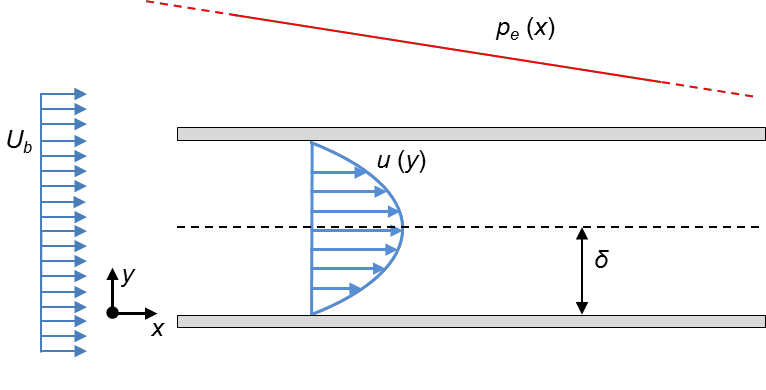
\includegraphics[width=\textwidth]{Case_Sketch.png}
                \centering
                \caption{Sketch of the Case}
                \label{fig:sketch}
        \end{figure}

        The configuration of the problem is as follows:
        \begin{itemize}
                \item Length \( L = 10 \: cm \),
                \item Length \( L_p = 9 \: cm \),
                \item Half-channel height \(\delta = 5 \: mm\),
                \item Bulk velocity \( U_b = 5 \: mm/s \),
                \item Fluid: Water at \( 20^{\circ}C \; ( \rho = 998.23 \: kg/m^3\), \\ Kinematic Viscosity \( \nu = 1.006E-6 \: m^2/s ) \).
        \end{itemize}

        \begin{figure}[!ht]
                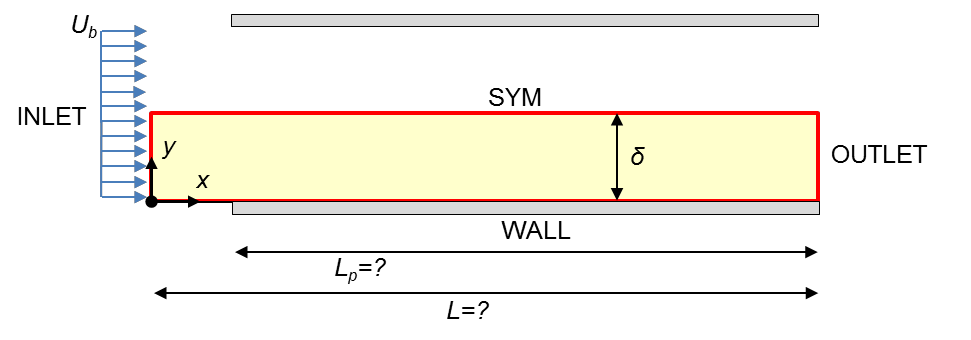
\includegraphics[width=\textwidth]{Conditions.png}
                \centering
                \caption{Domain and boundary conditions}
                \label{fig:conditions}
        \end{figure}

        \paragraph{Outline}
        The remainder of the report is organized as follows: Section~\ref{sec:developed_flow} provides some gross estimate of the required \( L_p \) to achieve a fully-developed flow in terms of channel height; Section~\ref{sec:independence} shows how a suitable configuration of the cartesian computational mesh was found; Section~\ref{sec:CFD_validation} compares the simulated solution with the analytical model both graphically and numerically; Finally, Section~\ref{sec:vorticity} provides some analysis regarding the vorticity profile on both the developing and fully-developed region. It is worth noting that all simulations had a relative convergence tolerance of $ 1E-3 $ for all variables taken into consideration.

\section{Fully-developed flow conditions} \label{sec:developed_flow}

        The following plot was generated from a half-domain simulation with a 40-by-40 mesh, in a $ 12 \: cm $ long domain with a $ 2 \: cm $ margin, as per the lab document's recommendation. The observed profile was taken in

        \begin{figure}[!ht]
                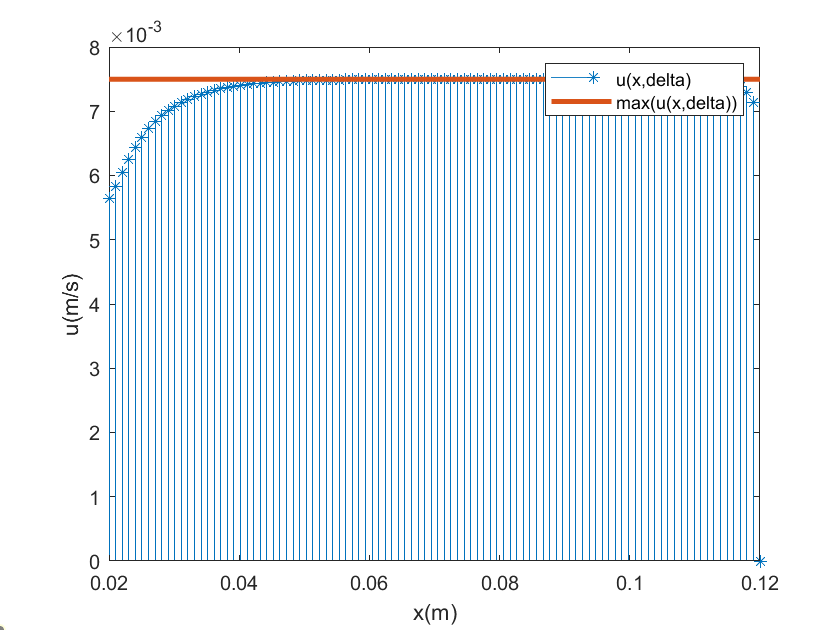
\includegraphics[width=\textwidth]{Fully_Developed_Francesco.png}
                \centering
                \caption{X-velocity Y-profile per delta-step}
                \label{fig:delta-steps}
        \end{figure}

        As we can see in Figure~\ref{fig:delta-steps}, the X-velocity Y-Profile stabilizes after roughly 4 deltas ($ 2 \: cm $), making our choice of an 18-delta channel with a 2-delta margin at the beginning ($ 10 \: cm $ total) more than enough for the case of study. From now on, unless said otherwise, all X-specific data was taken after 12 deltas into the actual channel ($ 7 \: cm $ from the origin of the X-axis), simulating the whole channel as opposed to just the lower half and using a \( 10 \: cm \) domain with a \( 1 \: cm \) margin in its stead.

\section{Grid independence study} \label{sec:independence}

        The following Grid-Independence study was performed by fixing 40 cells either along the X or Y axis, and then progressively increasing the amount of cells on the other axis until both X-velocity profile and Pressure-gradient convergence was observed.

        \begin{figure}[!ht]
                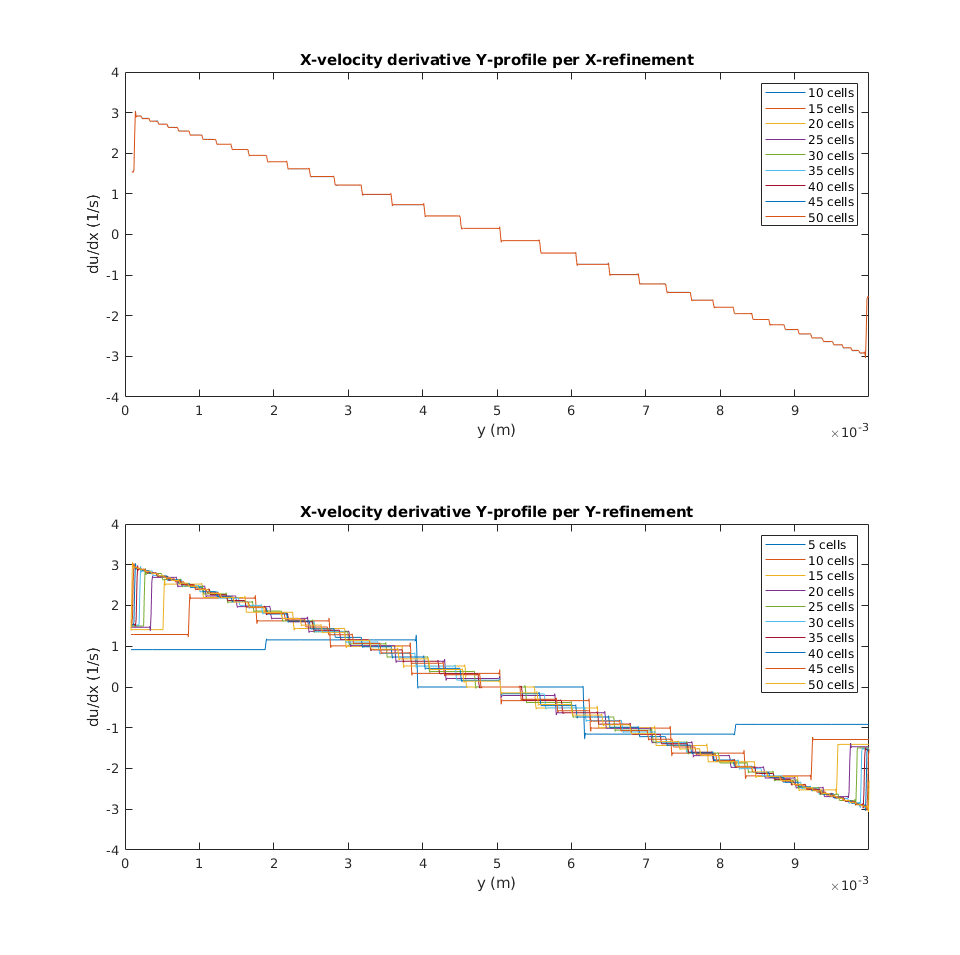
\includegraphics[width=\textwidth]{Grid_Ind_U_Profiles.png}
                \centering
                \caption{X-velocity derivative Y-profile per cell amount}
                \label{fig:grid_ind_u}
        \end{figure}

        \begin{figure}[!ht]
                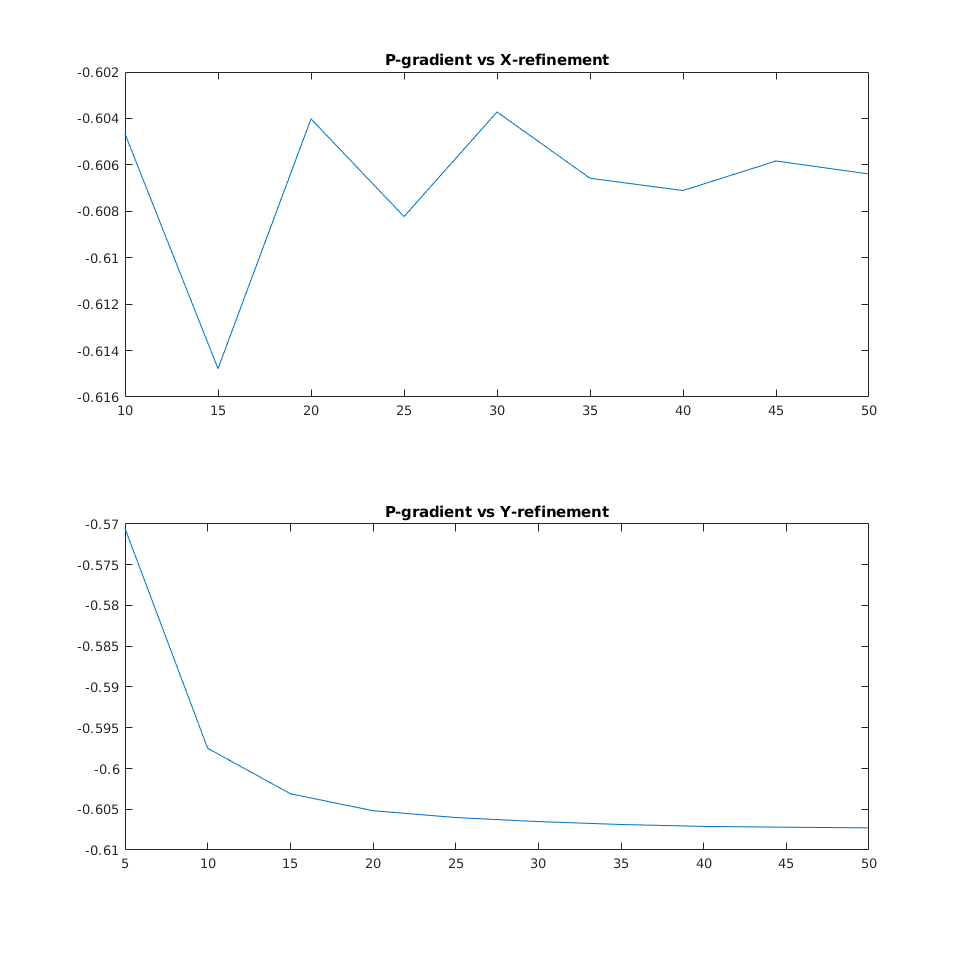
\includegraphics[width=\textwidth]{Grid_Ind_P_Gradient.png}
                \centering
                \caption{P-gradient vs cell amount}
                \label{fig:grid_ind_p}
        \end{figure}

        As we can observe in Figure~\ref{fig:grid_ind_u}, X-refinement is pretty much irrelevant for the X-velocity derivative profile; nevertheless, such is not the case for the Pressure-gradient which, as we can see in Figure~\ref{fig:grid_ind_p}, did not stabilize after at least 35 cells across the X-axis.

        In the case of Y-refinement, 25 cells were enough to stabilize both the X-velocity derivative profile and average Pressure-gradient. Therefore, a 40-by-40 mesh kept being used for the remainder of the laboratory, since simulation times were low enough for a wide Y-refinement margin to not be a problem.

\section{CFD solution validation} \label{sec:CFD_validation}

        From Equation System~\ref{eq:system} and Equation~\ref{eq:bulk_speed} (which describes Bulk velocity as a function of the Pressure-gradient magnitude), we derive the expressions in Equation System~\ref{eq:analytical}.

        \begin{equation} \label{eq:bulk_speed}
                U_b = - \frac{1}{3 \mu} \frac{dp_e}{dx} \delta ^ 2 
        \end{equation}

        \begin{equation} \label{eq:analytical}
                \begin{cases}
                        \frac{dp_e}{dx} = - \frac{3 \mu}{\delta ^ 2} U_b \\
                        u(y) = - \frac{\delta}{2 \mu} \frac{dp_e}{dx} y (2 - \frac{y}{\delta})
                \end{cases}
        \end{equation}

        In order to objectively measure the simulation error with respect to the analytical solution, we use the expressions in Equation System~\ref{eq:errors}. It is worth noting that the velocities inside the $ L^2 $-norm and $ L^{\infty} $-norm were evaluated for a fixed value of x inside the fully-developed region.

        \begin{equation} \label{eq:errors}
                \begin{cases}
                        \frac{dp}{dx}_{err} = \frac{\left| \frac{dp_e}{dx} - \frac{dp_e}{dx}_{sim} \right|}{\left| \frac{dp_e}{dx} \right|} \\
                        u_{err, L^2} = \frac{\left| \left| \frac{u - u_{sim}}{u} \right| \right|_{L ^ 2}}{\sqrt{2 \delta}} = \sqrt{\frac{\int_{0}^{2 \delta} \left| \frac{u(y) - u_{sim}(y)}{u(y)} \right|^2 dy}{2 \delta}} \\
                        u_{err, L^{\infty}} = \left| \left| \frac{u - u_{sim}}{u} \right| \right|_{L ^ \infty} = \sup_{y \in [0, 2 \delta]} \left| \frac{u(y) - u_{sim}(y)}{u(y)} \right|
                \end{cases}
        \end{equation}

        The results were the following:

        \begin{itemize}
                \item Pressure-gradient relative error: \( 5.807746E-03 \).
                \item X-velocity relative Root-Mean-Squared error: \( 5.288724e-03 \).
                \item X-velocity relative Maximum error: \( 2.613112e-02 \).
        \end{itemize}

        Aditionally, as we can observe in Figure~\ref{fig:u_comparison} and Figure~\ref{fig:tau_comparison}, the profiles for both X-velocity and Shear-stress were coherent with the analytical model.

        \begin{figure}[!ht]
                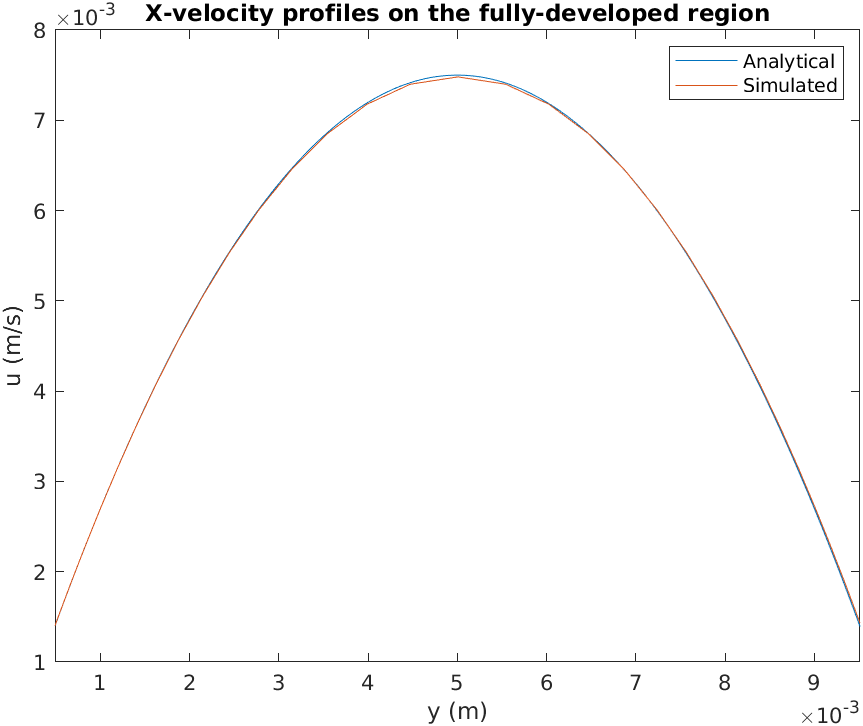
\includegraphics[width=\textwidth]{U_Profile_Comparison.png}
                \centering
                \caption{X-velocity profile comparison at \(x = 0.07 \: m \)}
                \label{fig:u_comparison}
        \end{figure}

        \begin{figure}[!ht]
                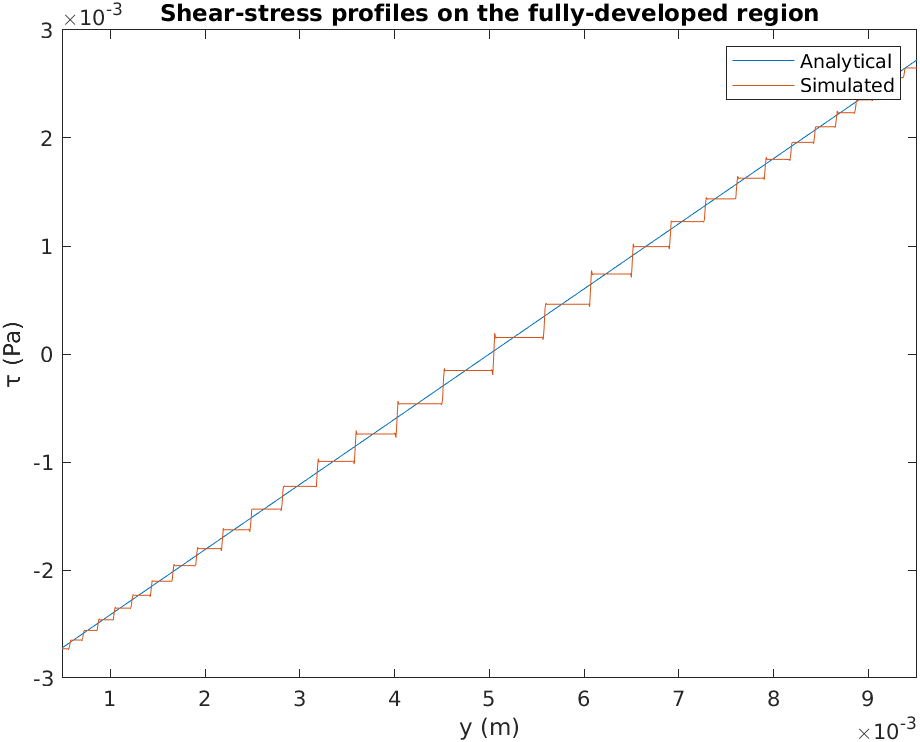
\includegraphics[width=\textwidth]{Tau_Profile_Comparison.png}
                \centering
                \caption{Shear-stress profile comparison at \(x = 0.07 \: m \)}
                \label{fig:tau_comparison}
        \end{figure}

\section{Vorticity} \label{sec:vorticity}

        Using data from the original simulation (for visualization purposes) and a 100-by-40 mesh, we plotted vorticity across all channel regions and obtained Figure~\ref{fig:vorticity} as a result.

        \begin{figure}[!ht]
                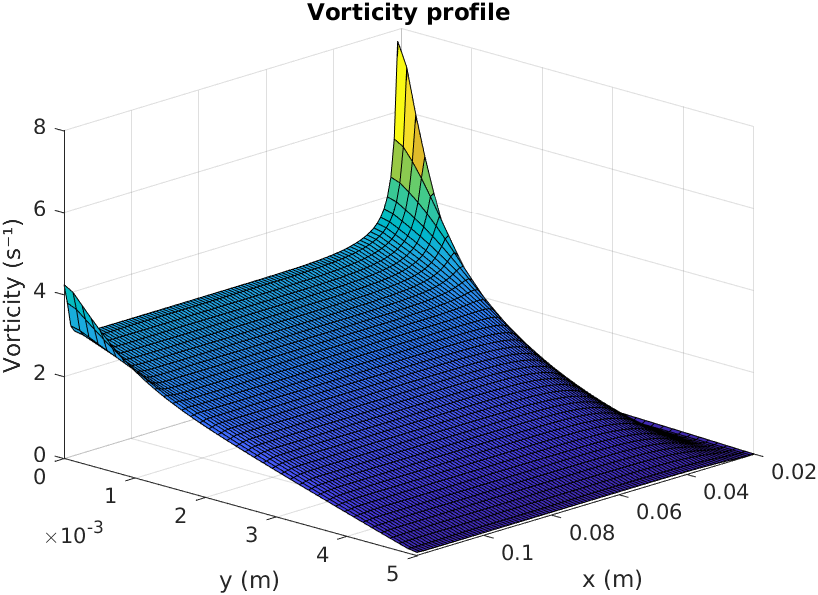
\includegraphics[width=\textwidth]{Vorticity_Profile_Francesco.png}
                \centering
                \caption{Vorticity surface-profile}
                \label{fig:vorticity}
        \end{figure}

        The main two differences between the developing and fully-developed regions are:

        \begin{itemize}
                \item Peak vorticity magnitude is higher on the developing region.
                \item The vorticity profile is completely linear on the fully-developed region, whereas it presents variable slope on the developing one.
        \end{itemize}

\bibliographystyle{abbrv}
\bibliography{main}

\end{document}
